% Under Methods section
% --------------------------------------------------
\subsubsection{Al-Si Rapid Solidification}
% --------------------------------------------------
To accurately model Al-Si solidification, solidification velocity must
first be measured from experiments. Solidification was monitored in situ
with a Dynamic Transmission Electron Microscope (DTEM).
A thin film of Al-3 wt.\% Si is deposited on a silicon nitride surface with a
thickness of approximately 100 nm.
A laser melts the Al-Si film and after a 20 µs delay, an electron beam
pulsing at 2.5 µs intervals is transmitted through the sample. The
resulting beam is rastered across a detector, which captures nine frames
of the solidification at 120x
magnification in a single image (\ref{fig/raw-false-color}).
An automated
identification procedure was developed to calculate the solidification
velocity by identifying the rapidly solidifying melt pool in each frame,
fitting an ellipse to each of the melt pools,
and analyzing the change in size of the ellipses. This procedure consists of
a series of Python functions, mostly implemented using a set of
packages similar to the packages used in the AM simulator procedure:
\textit{imageio}, \textit{NumPy}, \textit{scikit-image},
\textit{matplotlib}, \textit{SciPy}.
The functions were executed in \textit{Jupyter}
notebooks to yield incremental results at each step for three separate DTEM
images depicting rapid solidification of Al-3 wt.\% Si.

\begin{figure}[ht]
    \centering
    \includegraphics[width=0.9\textwidth]{figures/04/04-raw-false-color.png}
    \caption{
        \small\setstretch{1}
        (a) Dynamic transmission electron microscope (DTEM) image showing
        nine frames of a rapidly solidifying Al-3 Si sample with a 20 µs
        delay and 2.5 µs capture interval. The chronology of the experiment
        starts with the lower right image, moves up the right column, down
        the center column, and finally up the left column to end at the top
        left image.
        (b) The same image with false color highlighting intensity
        differences across the image.
    }
    \label{fig/raw-false-color}
\end{figure}

\subsubsection{Rapid Solidification Detection Procedure}
% --------------------------------------------------
The detection procedure consists of four parts:
preprocessing, morphologic operations, ellipse fitting, and analysis. In
the preprocessing routine, the DTEM image is separated into nine frames by
performing a lower minimum threshold to create a binary image. The binary
image contains masks of the nine elliptical frames, which are labeled
according to connected pixel region in the image using a \textit{scikit-image}.
The labeled image is passed to the \textit{scikit-image} function
\textit{measure.regionprops}, which provides information necessary to crop
each of the nine frames and center them into nine separate images of matching
size. For each of
these separated frames, a pseudo-flat-field image is created by smoothing
the image with a large Gaussian filter and replacing the background pixels
(beyond the elliptical frame) with the mean intensity of the image
(\ref{fig/raw-flatfield}). Each resulting pseudo-flat-field image is
used to normalize each frame, smoothing out localized intensity fluctuations.
This pseudo-flat-field correction is performed for each of the nine frames
(\ref{fig/raw-rescaled}).

\begin{figure}[ht]
    \centering
    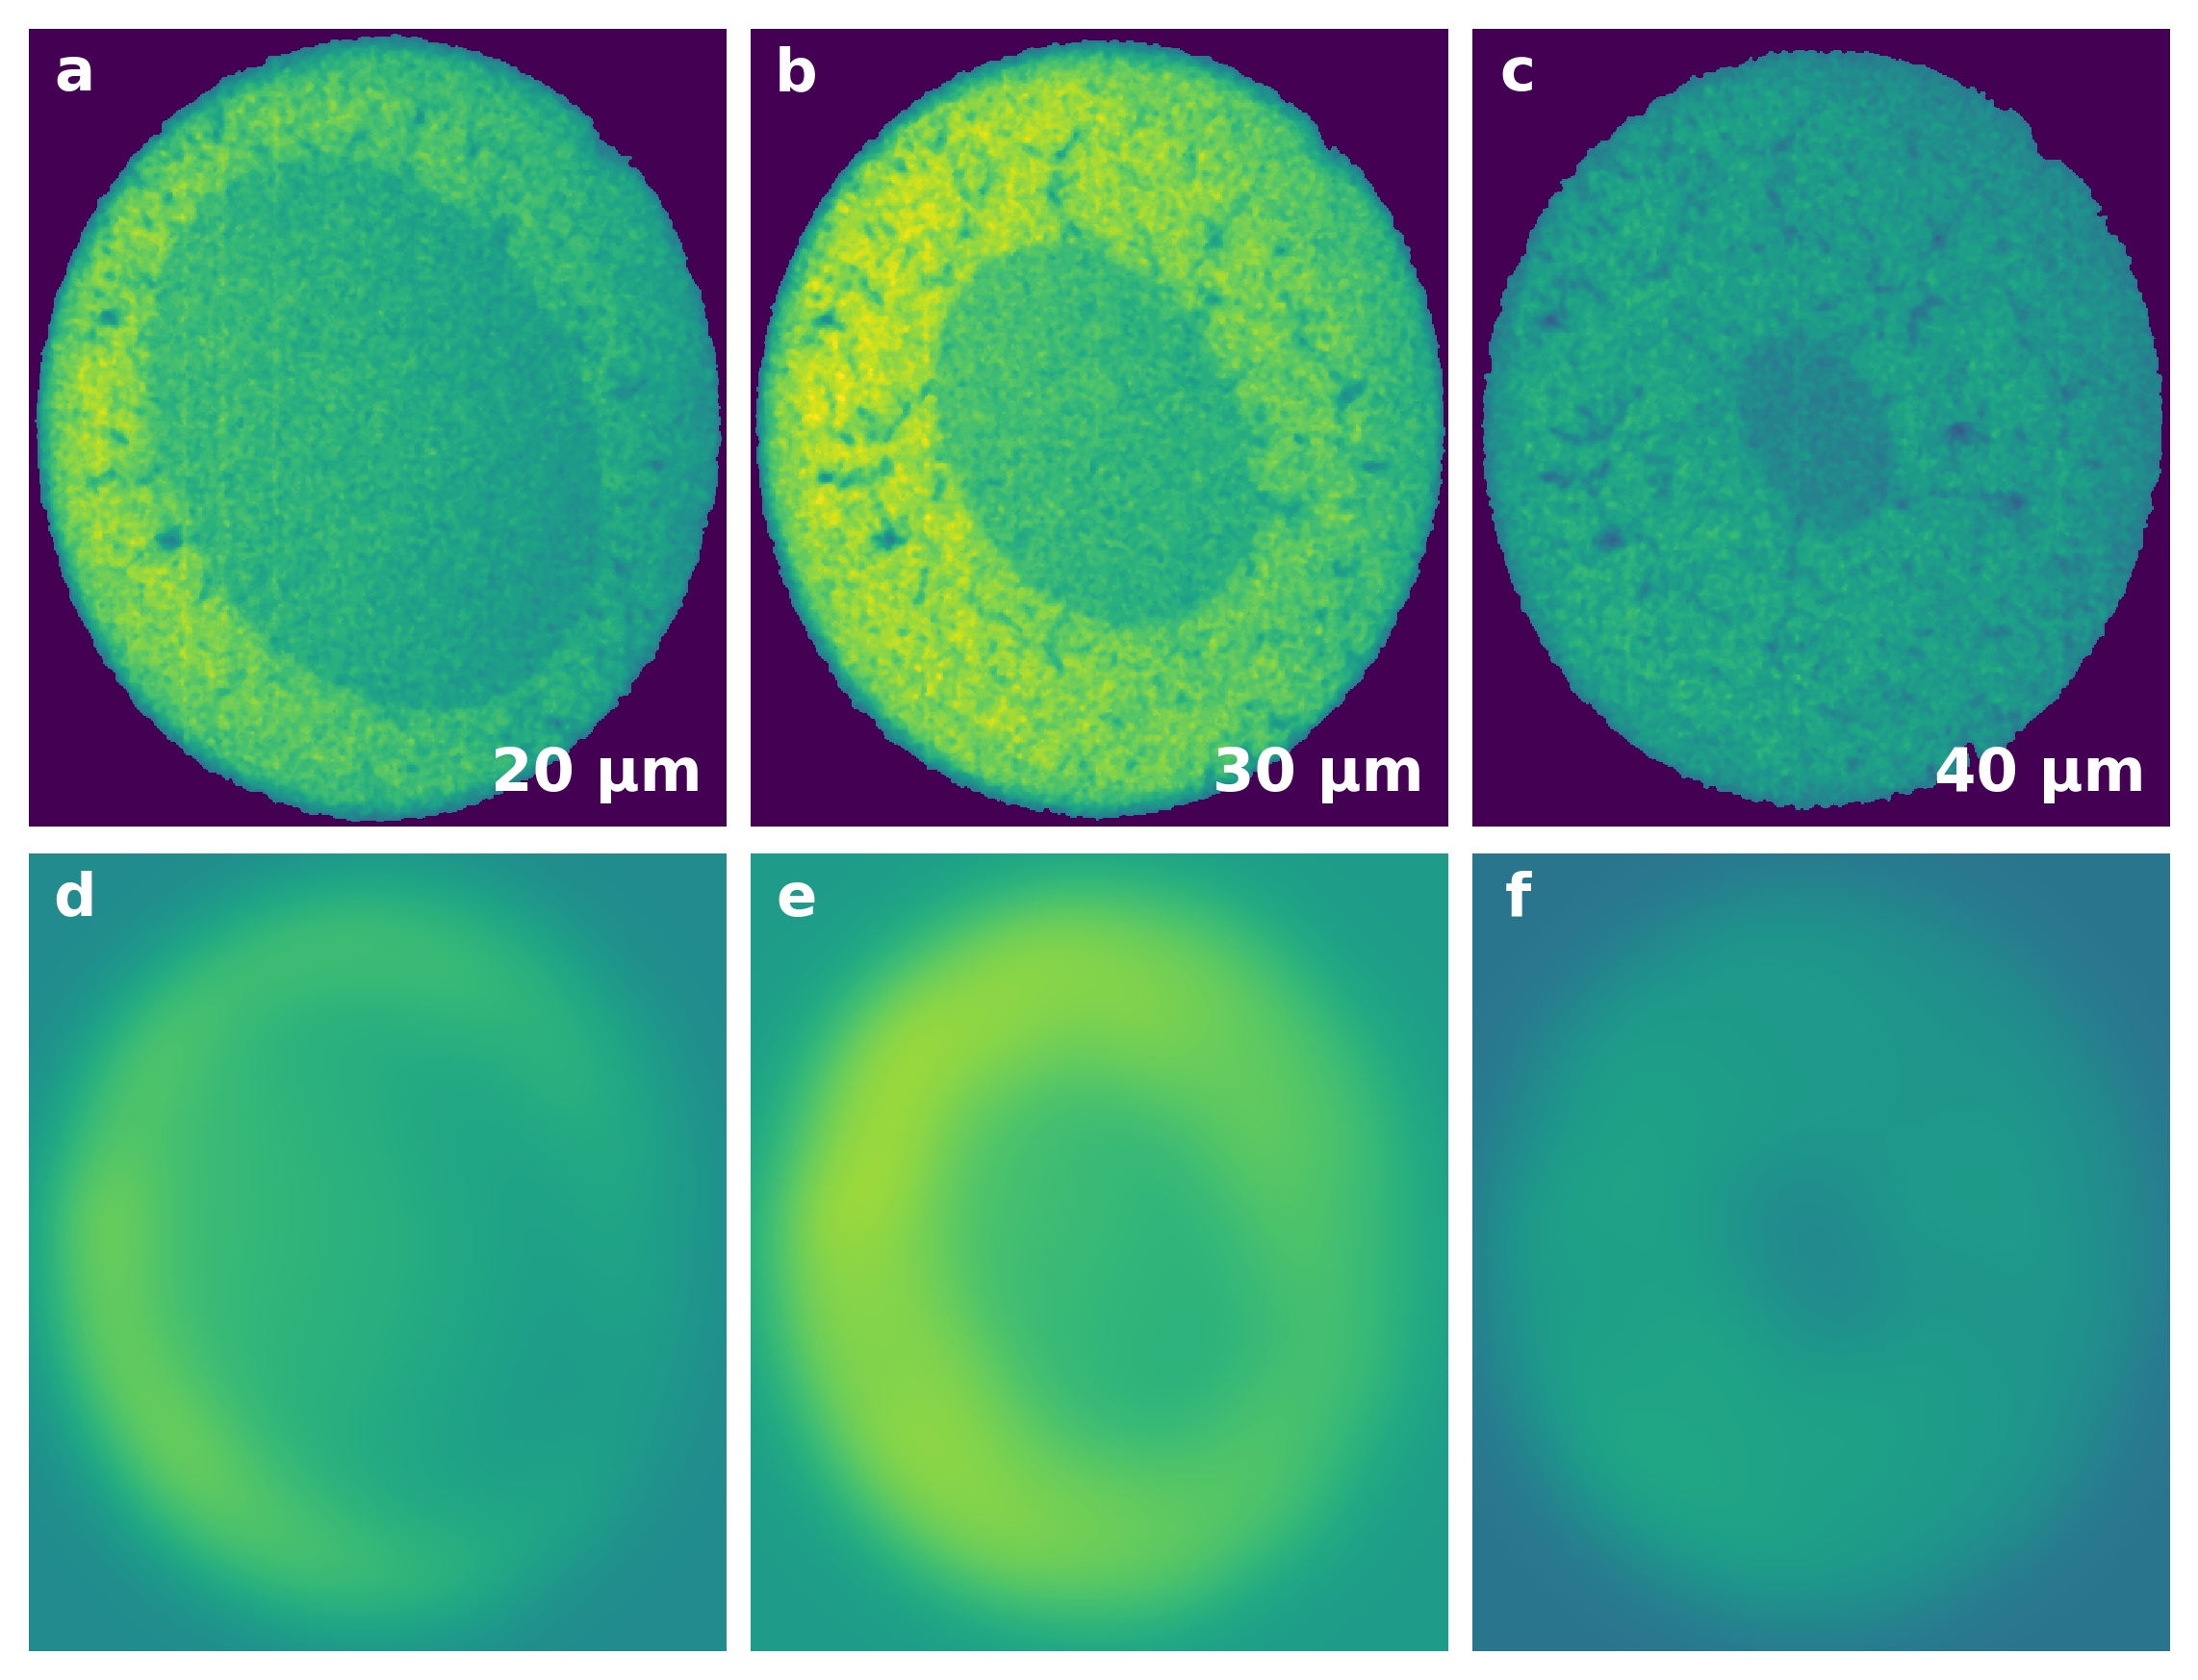
\includegraphics[width=0.6\textwidth]{figures/04/05-raw-flatfield.png}
    \caption{
        \small\setstretch{1}
        (a - c) Subset of frames with intensity unchanged following
        extraction from full DTEM image. Frames correspond to 20 µs, 30 µs,
        and 40 µs after the laser melted the sample.
        (d - f) Pseudo flat-field images created with large-sigma Gaussian
        filter and mean-filled background.
        Created from corresponding frames (a - c).
    }
    \label{fig/raw-flatfield}
\end{figure}

\begin{figure}[h]
    \centering
    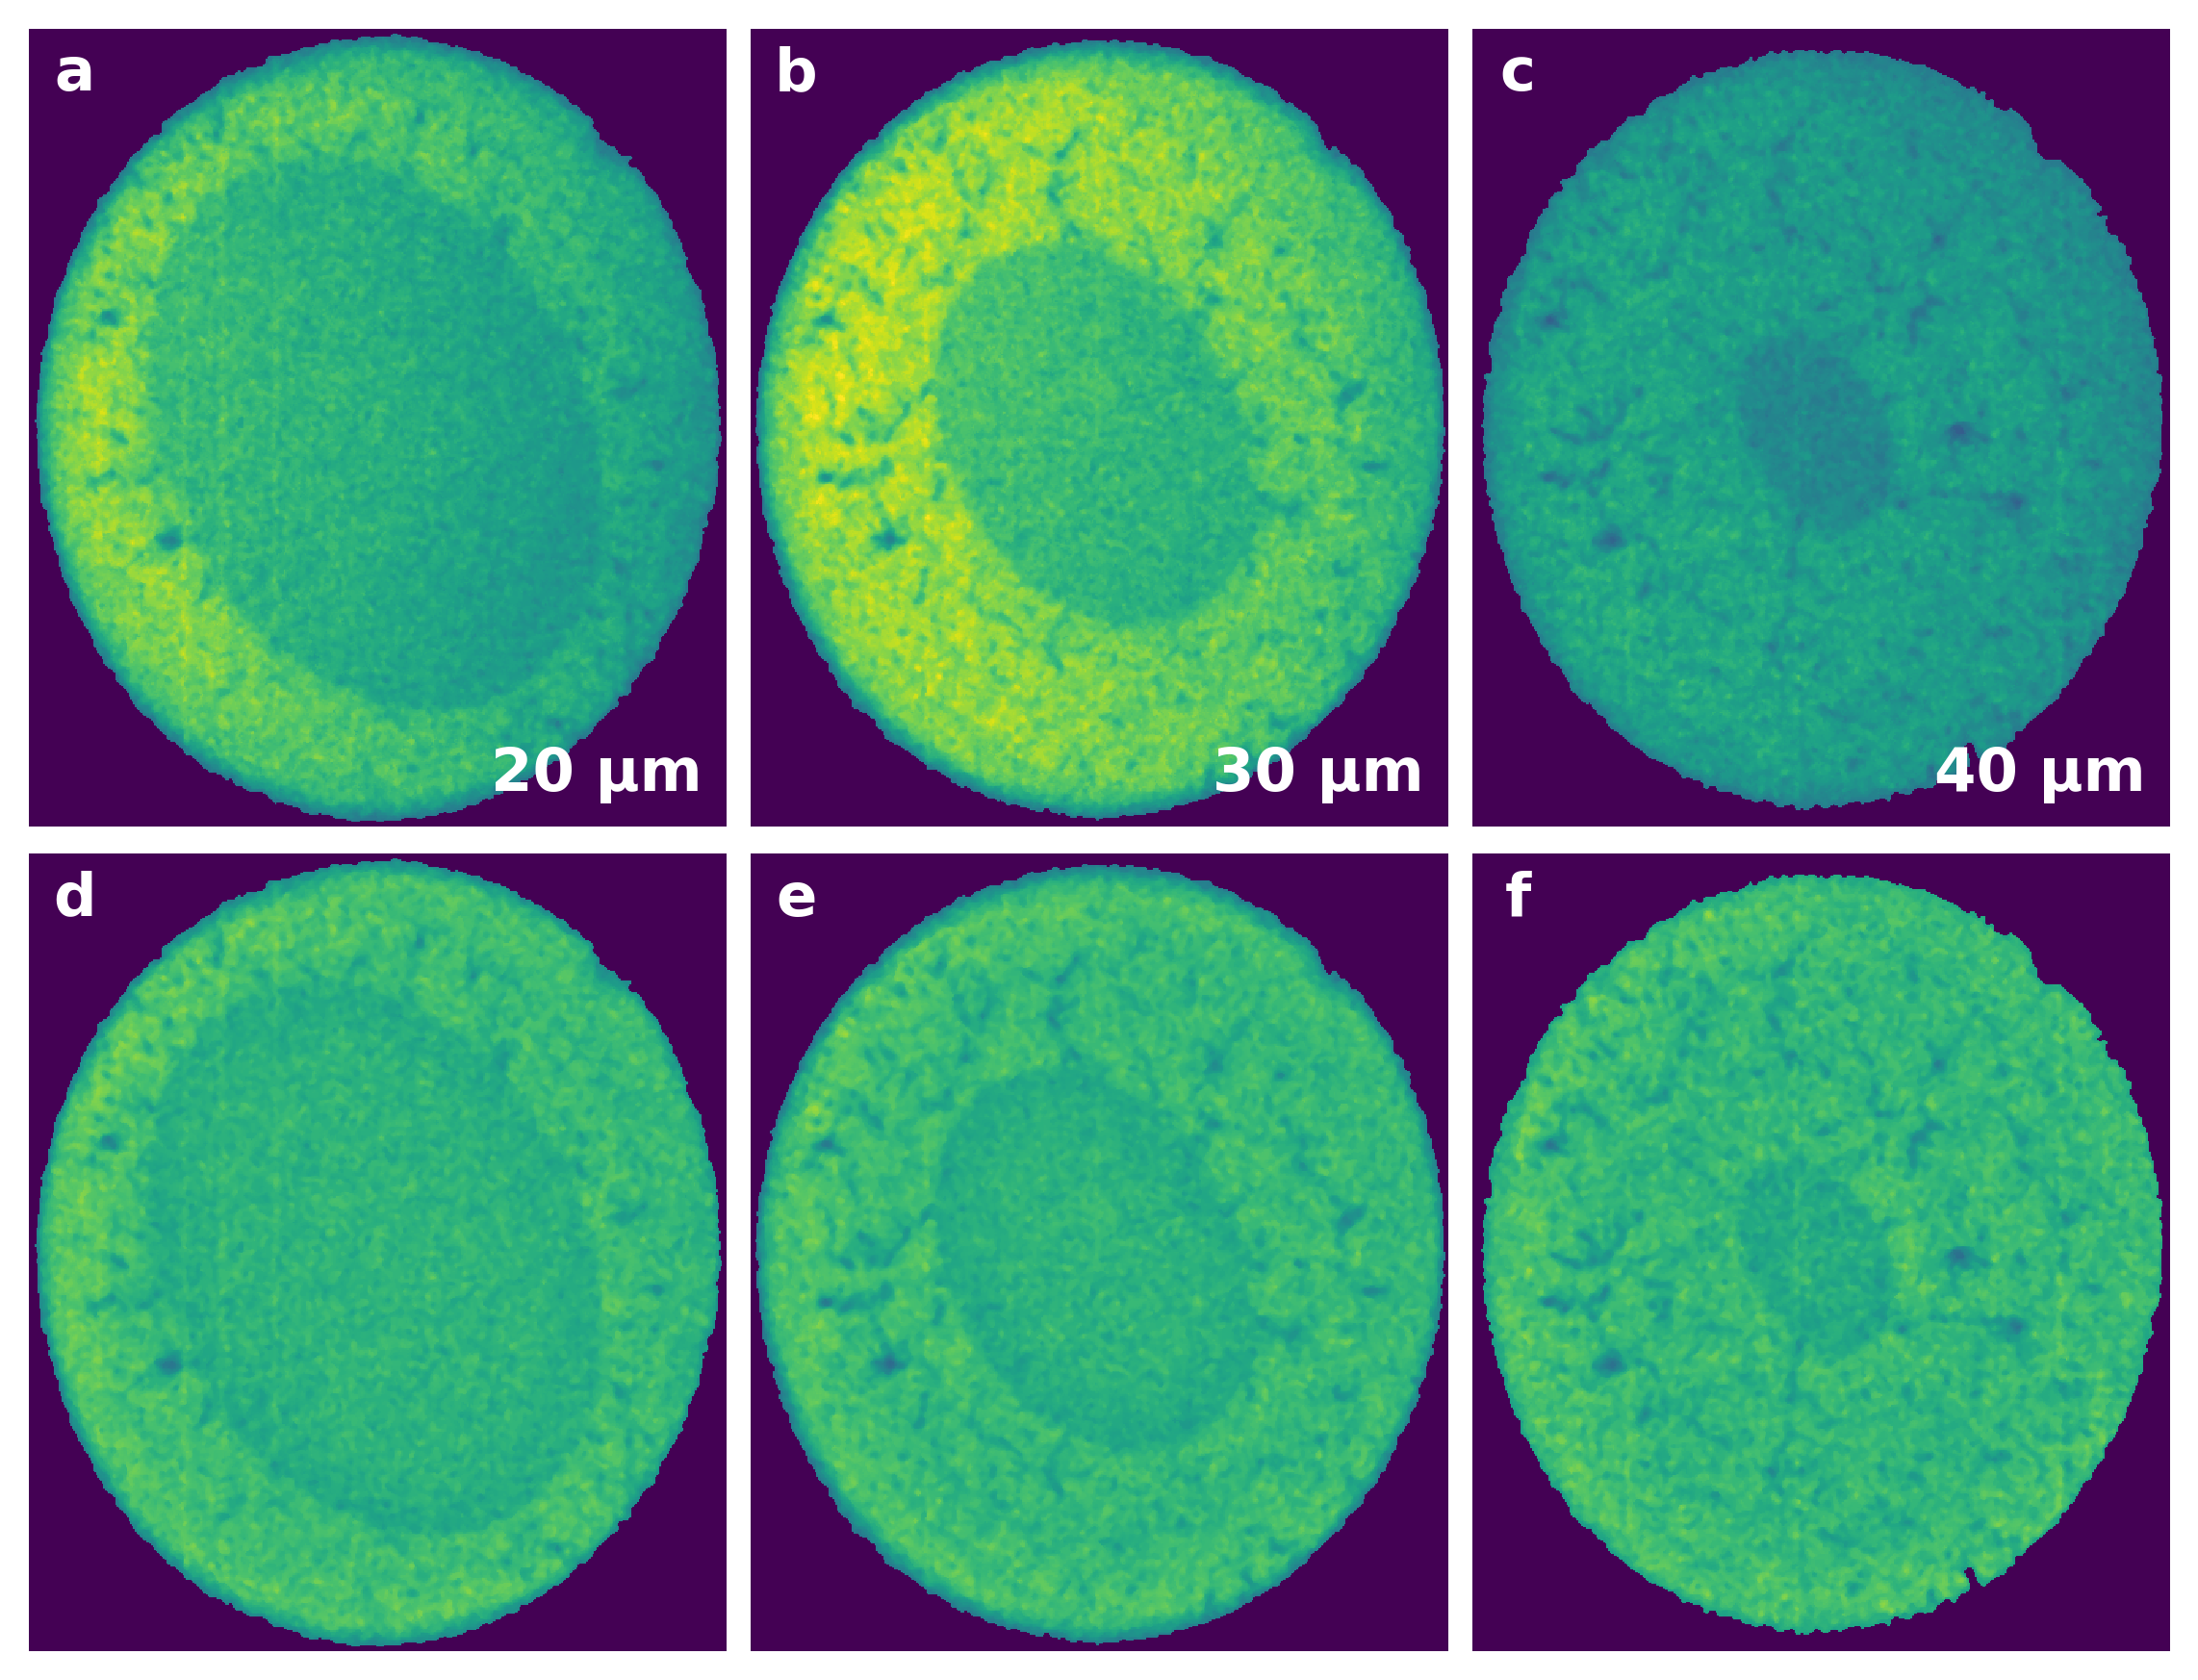
\includegraphics[width=0.6\textwidth]{figures/04/06-raw-rescaled.png}
    \caption{
        \small\setstretch{1}
        Comparison between raw DTEM frames and intensity-rescaled frames
        following pseudo-flat-field correction.
        (a - c) Subset of frames with intensity unchanged following
        extraction from full DTEM image. Frames correspond to 20 µs, 30 µs,
        and 40 µs after the laser melted the sample.
        (d - f) Subset of frames following pseudo flat-field images created
        with large-sigma Gaussian filter and mean-filled background.
        Created from corresponding frames as (a - c) and pseudo flat-field
        images (\ref{fig/raw-flatfield}.d - f).
    }
    \label{fig/raw-rescaled}
\end{figure}

Following the pseudo-flat-field correction, the rescaled frames are then
subjected to the morphologic operation stage of the procedure. An upper
minimum threshold is used to create a binary image (\ref{fig/morpho}.a),
on which morphologic opening is performed to sever connections across the melt
pool. With regions disconnected, regions smaller than the mean region size
are removed from the binary image (\ref{fig/morpho}.b), then the image
is inverted and regions at the border of the image are removed
(\ref{fig/morpho}.c). At this point, the largest region is selected
(\ref{fig/morpho}.d) and morphologic closing is performed to close any
remaining gaps across the area corresponding to the S-L interface
(\ref{fig/morpho}.e). Finally, all the holes inside the
remaining region are filled, to create a single, roughly elliptical shape
(\ref{fig/morpho}.f).

\begin{figure}[ht]
    \centering
    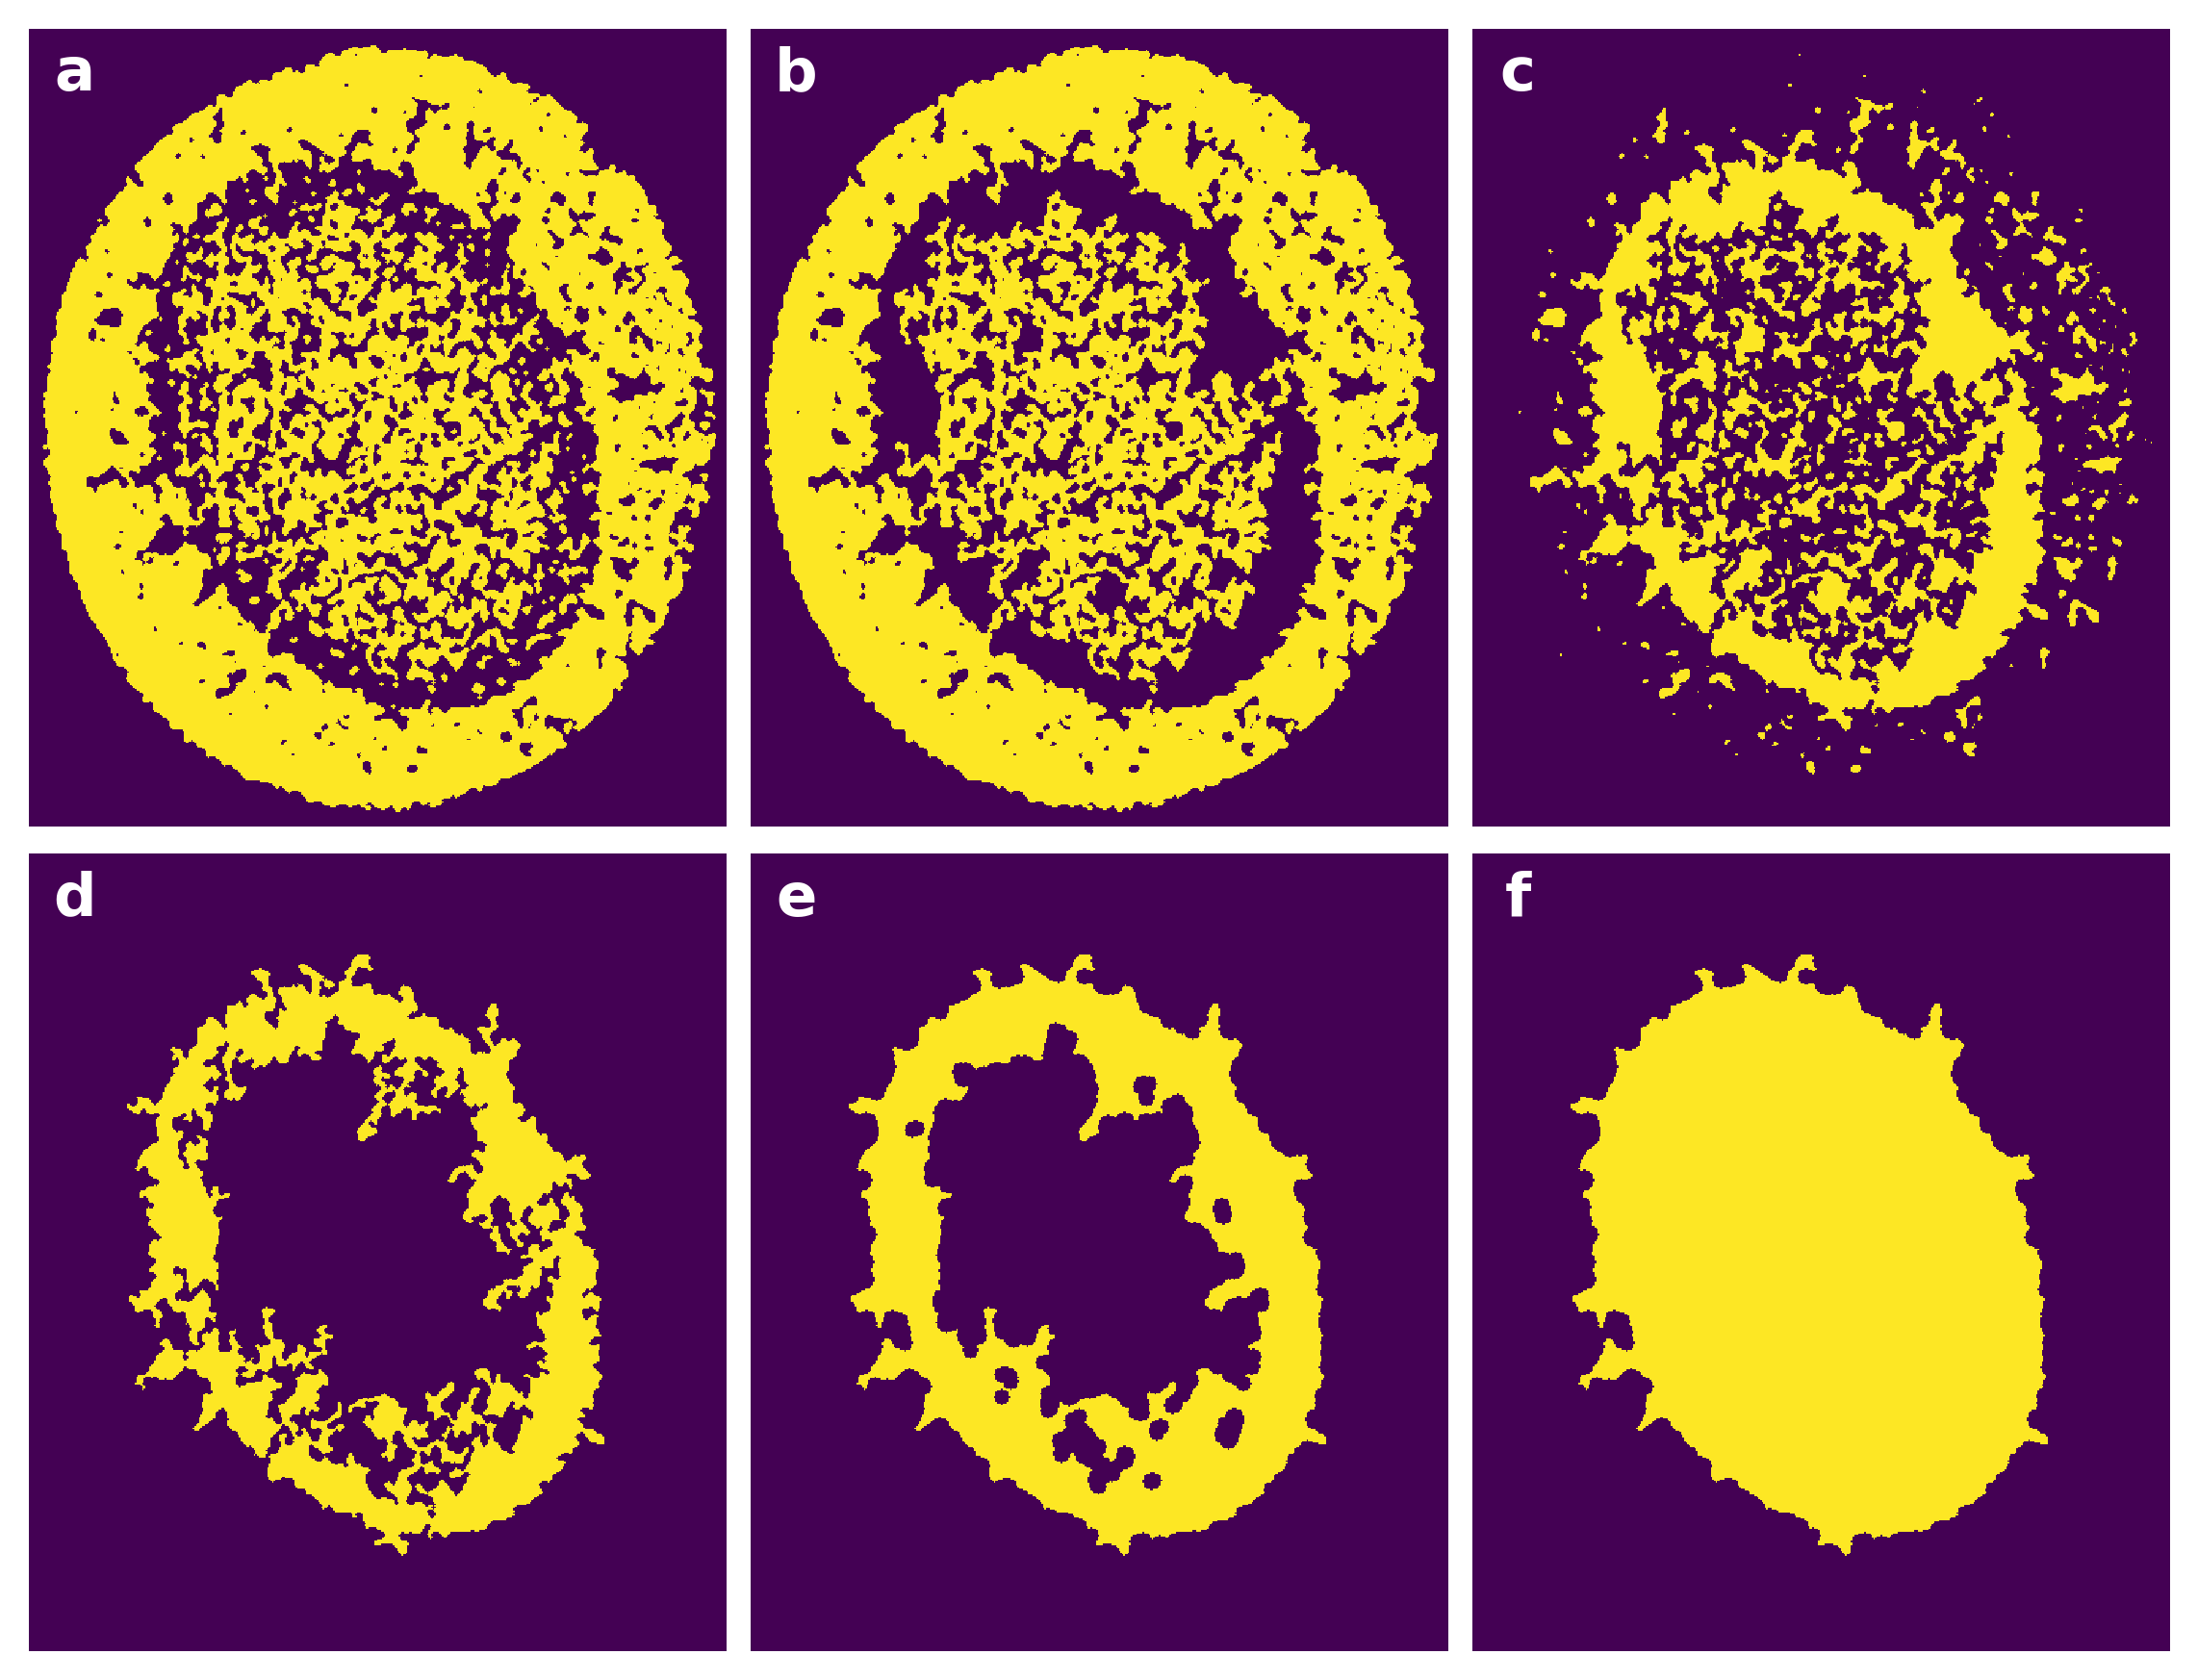
\includegraphics[width=0.6\textwidth]{figures/04/07-morpho.png}
    \caption{
        \small\setstretch{1}
        Series of morphological operations to automatically mask the
        liquid region of each solidifying frame from the DTEM image.
        (a) Upper minimum threshold of 20 µs frame
        (\ref{fig/raw-rescaled}.d).
        (b) Result of morphological opening of (a) to severe small
        connections across the solid-liquid interface followed by filtering
        of regions smaller than the mean area of all the regions present.
        (c) Inversion of b followed by removal of regions connected to the
        border.
        (d) Selection of region in (c) with largest area.
        (e) Morphological closing of (c) to connect small gaps across the
        solid-liquid interface that were not disconnected in the opening in (b).
        (f) Filling of all holes to create the final identified region.
    }
    \label{fig/morpho}
\end{figure}

This routine is performed for each frame, resulting in nine roughly
elliptical identified regions. These regions contain the melt pools,
though the masks contain artifacts branching off from the elliptical melt
pools that correspond to darker features around the edge of the true melt
pools (\ref{fig/rescaled-filled}).

\begin{figure}[ht]
    \centering
    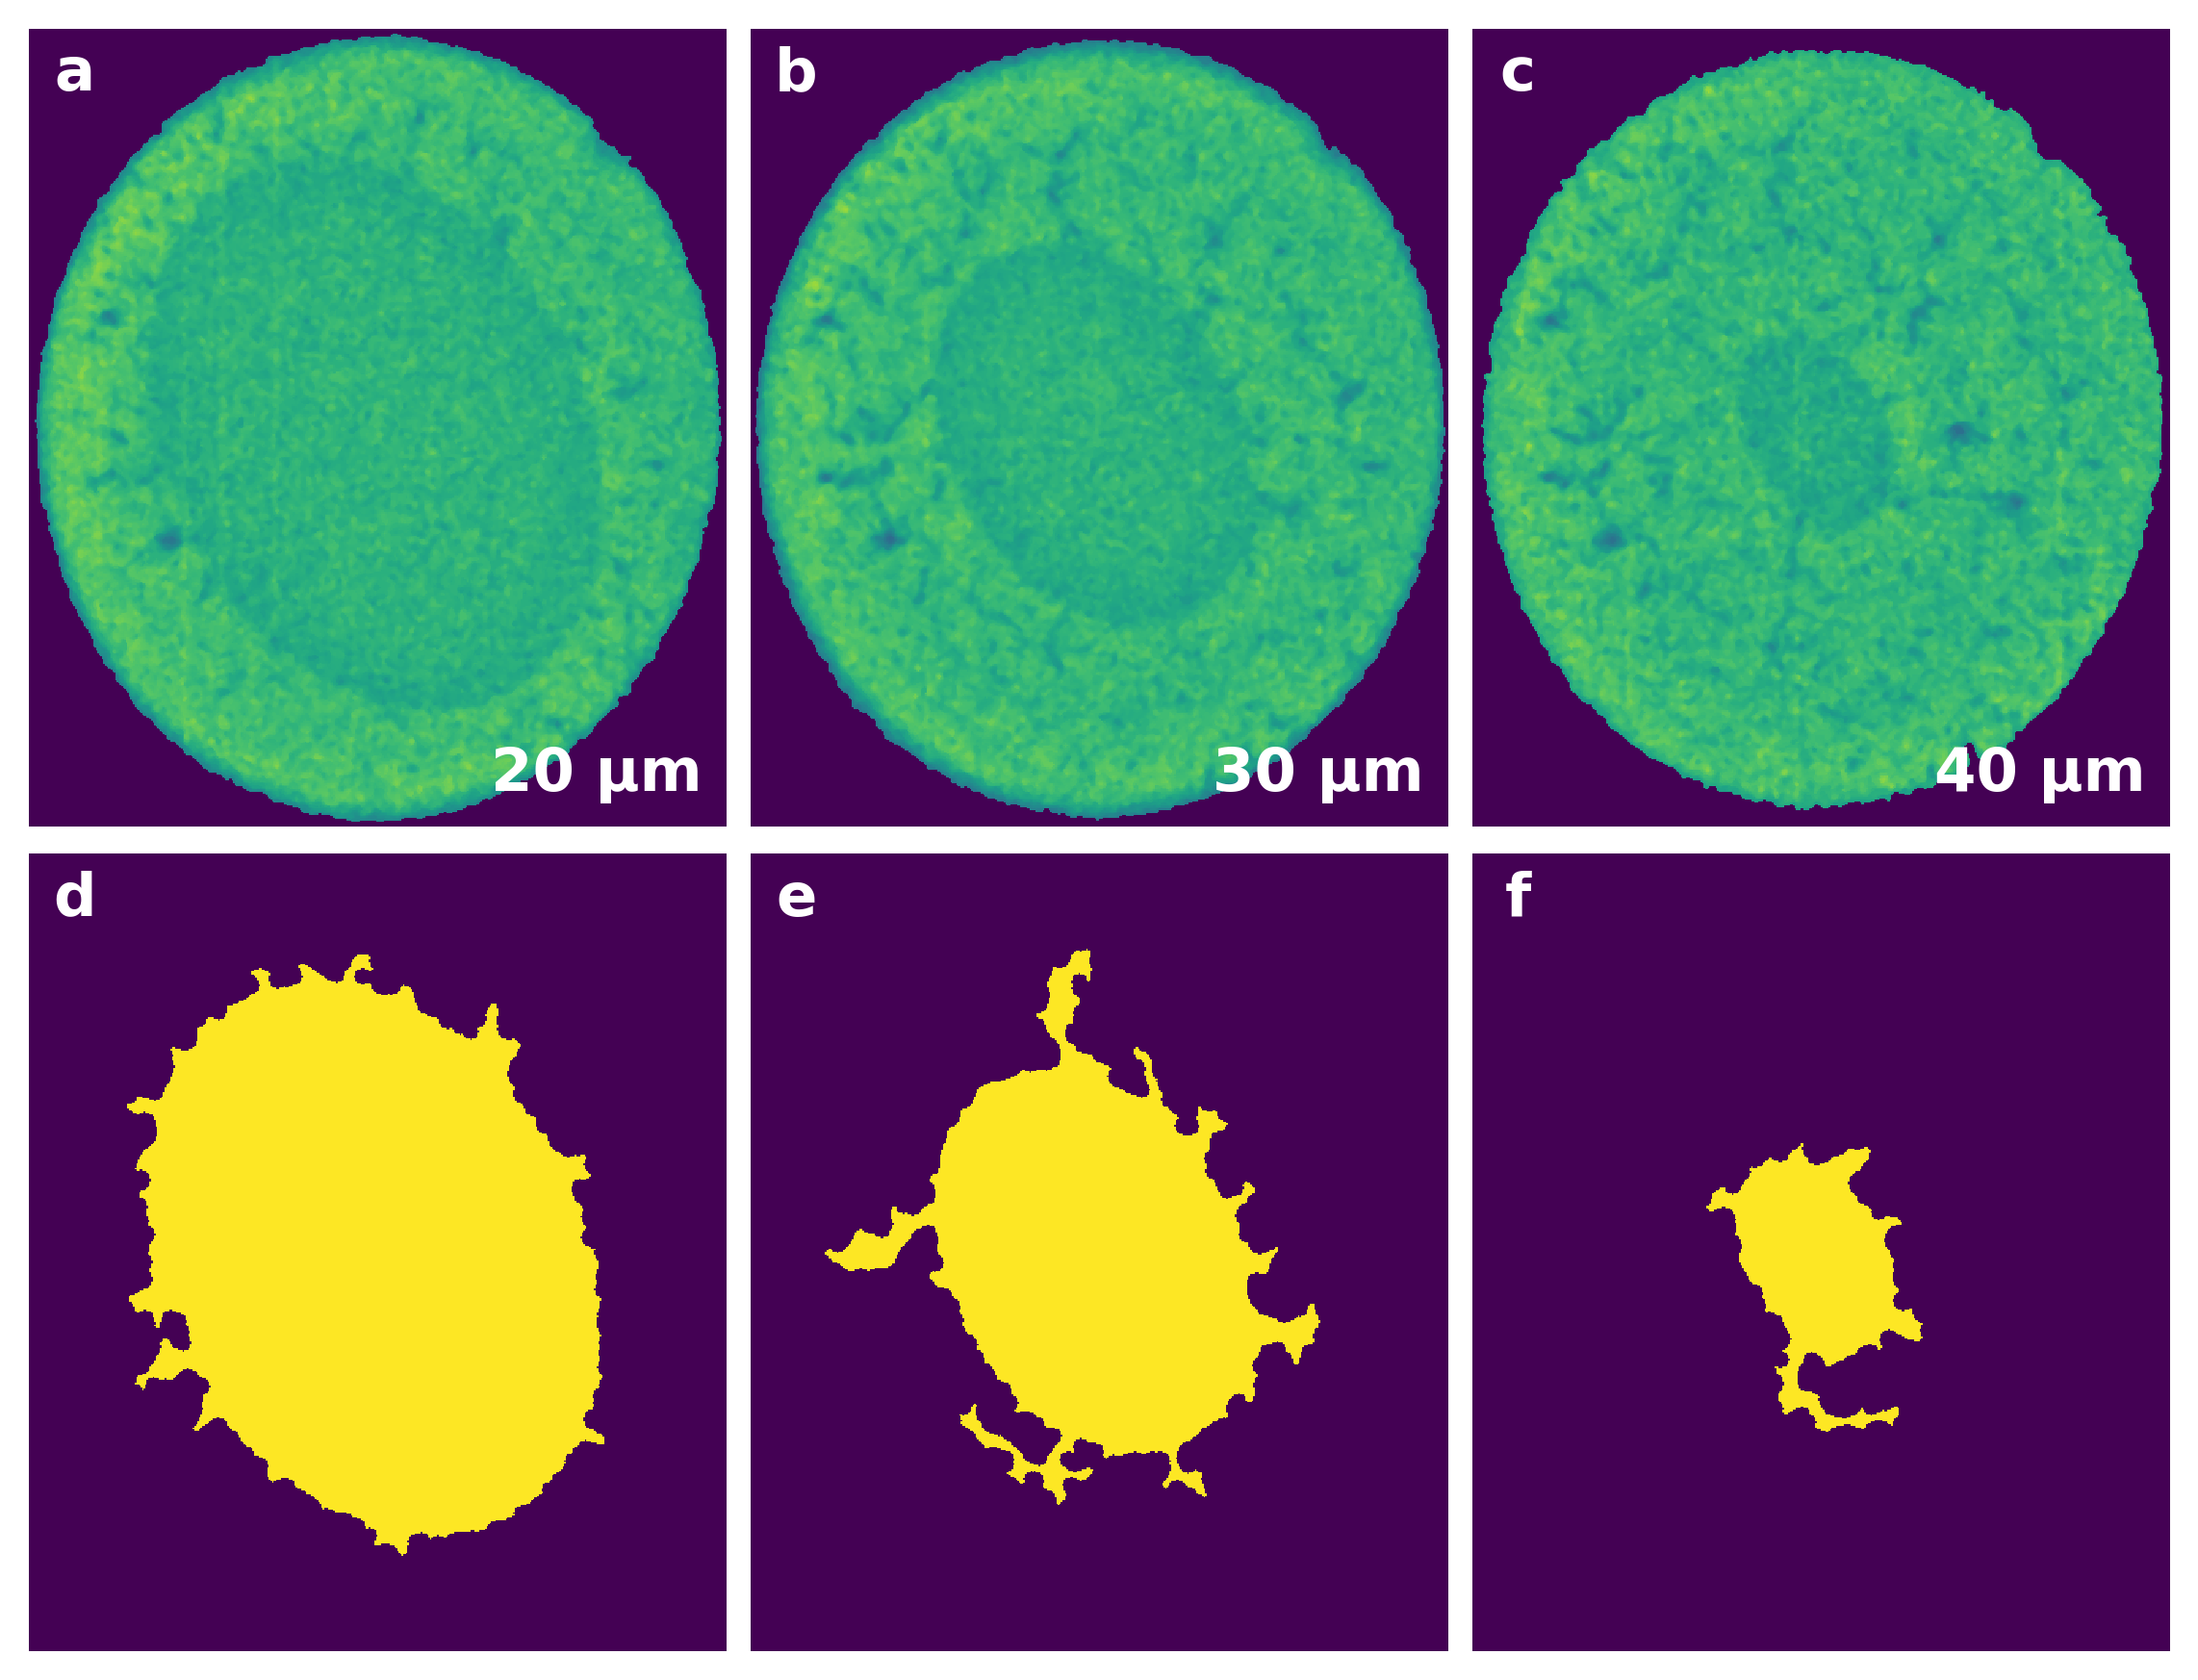
\includegraphics[width=0.6\textwidth]{figures/04/08-rescaled-filled.png}
    \caption{
        \small\setstretch{1}
        (a - c) Subset of normalized frames depicting Al-Si solidification
        20 µs, 30 µs, and 40 µs after the laser melted the sample.
        (d - f) Roughly elliptical identified regions containing the melt
        pools resulting from the series of morphologic operations
        (\ref{fig/morpho}.a - f)
        applied to each frame.
    }
    \label{fig/rescaled-filled}
\end{figure}

The ellipse fitting stage of the routine takes the identified region for
each frame and fits an ellipse to the region. An ellipse with the same
second moment as the identified region is calculated with the
\textit{scikit-image}
function \textit{measure.regionprops} as a first approximation fit. This
ellipse is rasterized onto an image of the same size as the
and at the same centroid as the identified region.
Both the fitted ellipse and the identified region are represented as binary
images with pixel intensities of either one or zero, so the mismatch
between the two images can be represented by the sum of the pixels shared
between the two images.
True fit pixels represent the pixels valued one in both images.
Misfit pixels represent the pixels valued valued zero in the
identified region but valued one in the fitted ellipse image.
Unfit pixels represent the pixels valued one in the identified regions but
valued zero in the fitted ellipse image.
Each of these types of pixels can be visualized by overlaying the fitted
ellipse image on the identified regions
and assigning different colors to different pixel types
(\ref{fig/rescaled-nonoptim}).

\begin{figure}[ht]
    \centering
    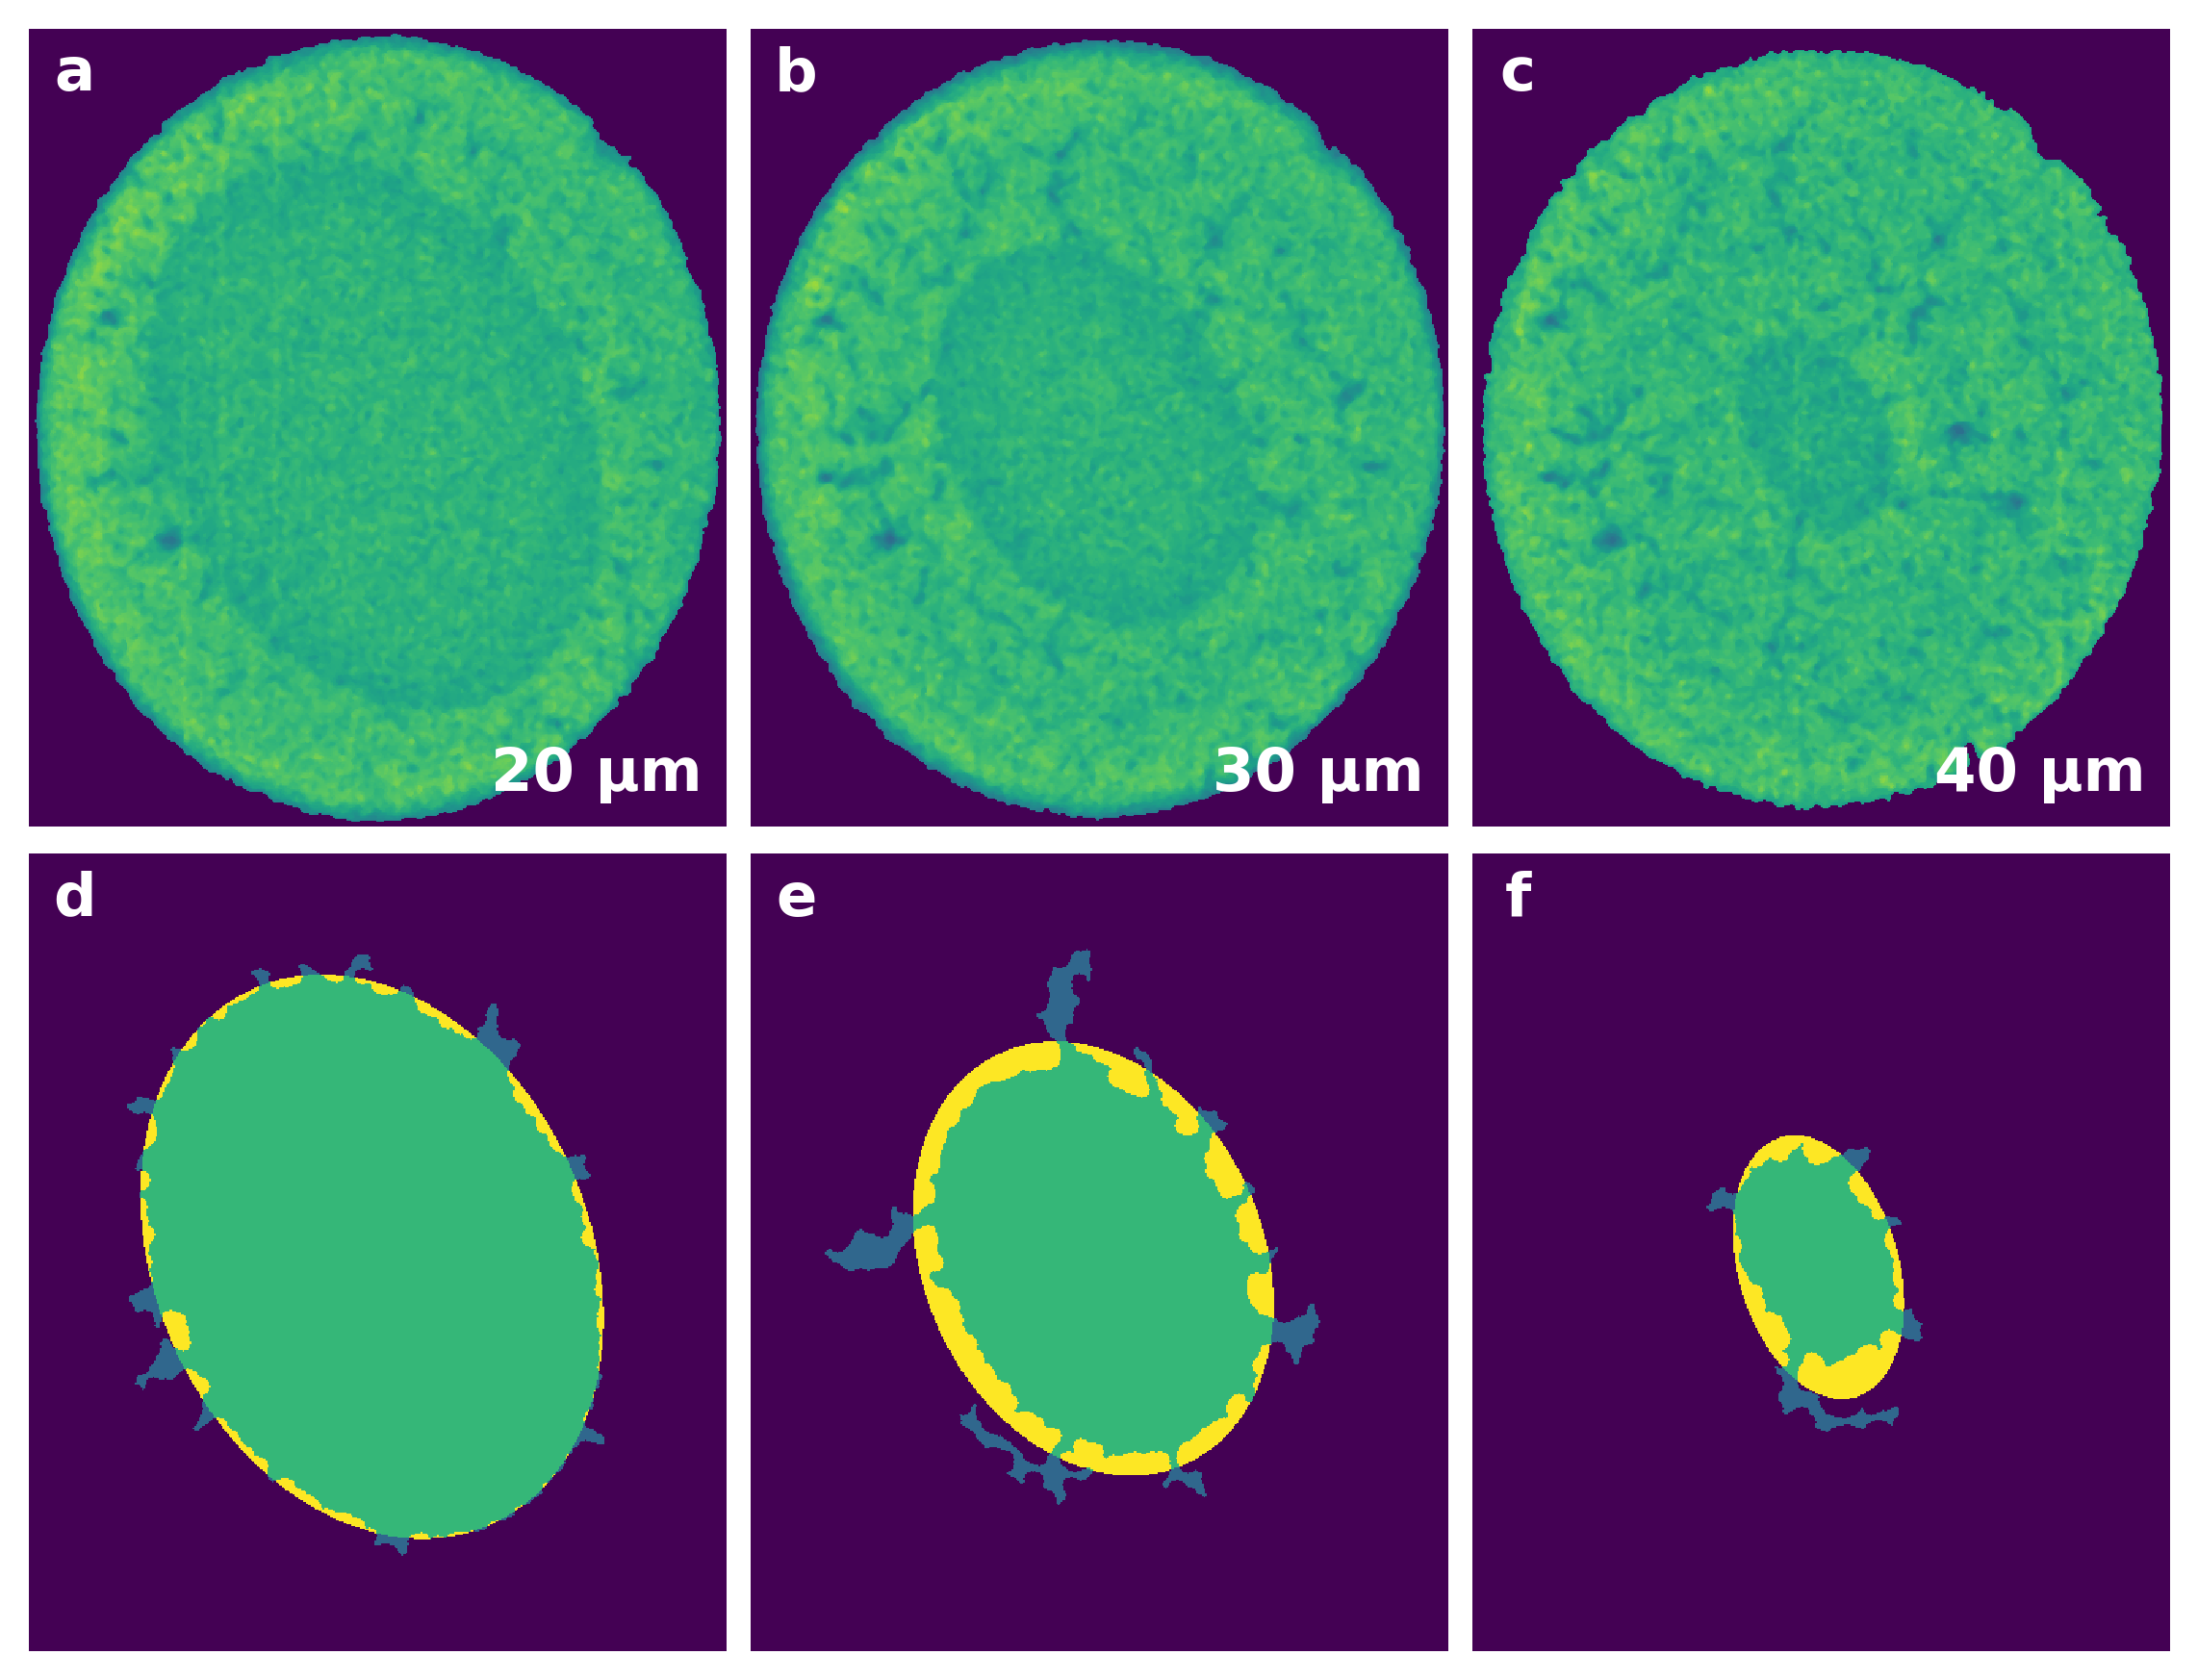
\includegraphics[width=0.6\textwidth]{figures/04/09-rescaled-nonoptim-fit.png}
    \caption{
        \small\setstretch{1}
        (a - c) Subset of normalized frames depicting Al-Si solidification
        20 µs, 30 µs, and 40 µs after the laser melted the sample.
        (d - f) Identified regions overlaid with fitted ellipses generated by
        finding ellipse parameters that match the centroid and second
        moment of the identified regions. The color of the pixels show the
        extent to which the fit matches the identified region.
        True fit pixels are within both the identified region and
        the ellipse (green), misfit pixels are beyond the identified
        region but still within the ellipse (yellow), and unfit pixels are
        beyond both the identified region and the ellipse (blue).
    }
    \label{fig/rescaled-nonoptim}
\end{figure}

The ellipse of equal second moment from \textit{scikit-image}
(\ref{fig/rescaled-nonoptim}) is used
as a starting point for fit optimization. The parameters defining the
ellipse (centroid x-coordinate, centroid y-coordinate, minor radius, major
radius, and orientation) are optimized using the downhill simplex
algorithm \cite{Nelder1965} implemented in \textit{SciPy} as the function
\textit{optimize.fmin}.
This function works by minimizing the value returned by a custom cost
function (Equation \ref{eqn/cost}) for a frame with $m$ rows and $n$
columns:
\begin{equation} \label{eqn/cost}
    cost =
    - \left(
        \sum_{i = 0}^{m}\sum_{j = 0}^{n} T_{ij}
    \right)
    \left(
        \sum_{i = 0}^{m}\sum_{j = 0}^{n} T_{ij}
        + \sum_{i = 0}^{m}\sum_{j = 0}^{n} M_{ij}
        + \frac{1}{4} \sum_{i = 0}^{m}\sum_{j = 0}^{n} U_{ij}
    \right)^{-1}
\end{equation}
where
$T$ represents a true fit pixel within both the identified region and the
fitted ellipse,
$M$ represents a misfit pixel beyond the identified region but within
the fitted ellipse, and
$U$ represents an unfit pixel beyond the identified region and the
fitted ellipse.
Including the sum of true fit pixels in the numerator and denominator
of the cost function means that a perfect fit would be a cost value of -1.
The addition of the sum of the misfit and unfit pixels in
the denominator decreases the cost value from -1 for additional pixels
that are mismatched between the fitted ellipse image and the identified
region. Since these terms are added to the sum of true fit pixels in
the denominator, the effect of each additional mismatched pixel acts
relative to the number of true fit pixels. For a frame with
larger true fit alignment, each individual mismatched pixel
contributes less to the overall cost value than the same mismatched pixel
would contribute to a frame with a smaller true fit alignment. The ¼
factor also reduces the contribution of unfit pixels, making true fit and
misfit pixels the most important factor in the cost
function, and therefore in the optimization process as a whole.

The outputted ellipse
parameters returned from the optimization process show an improvement in
the fit represented by a decrease in the sum of misfit and unfit pixels
(\ref{fig/rescaled-optim}).
It is interesting to note that most of the
unfit pixels do not appear to be part of the melt pool, but
instead correspond to darker regions of the solidified metal.

\begin{figure}[ht]
    \centering
    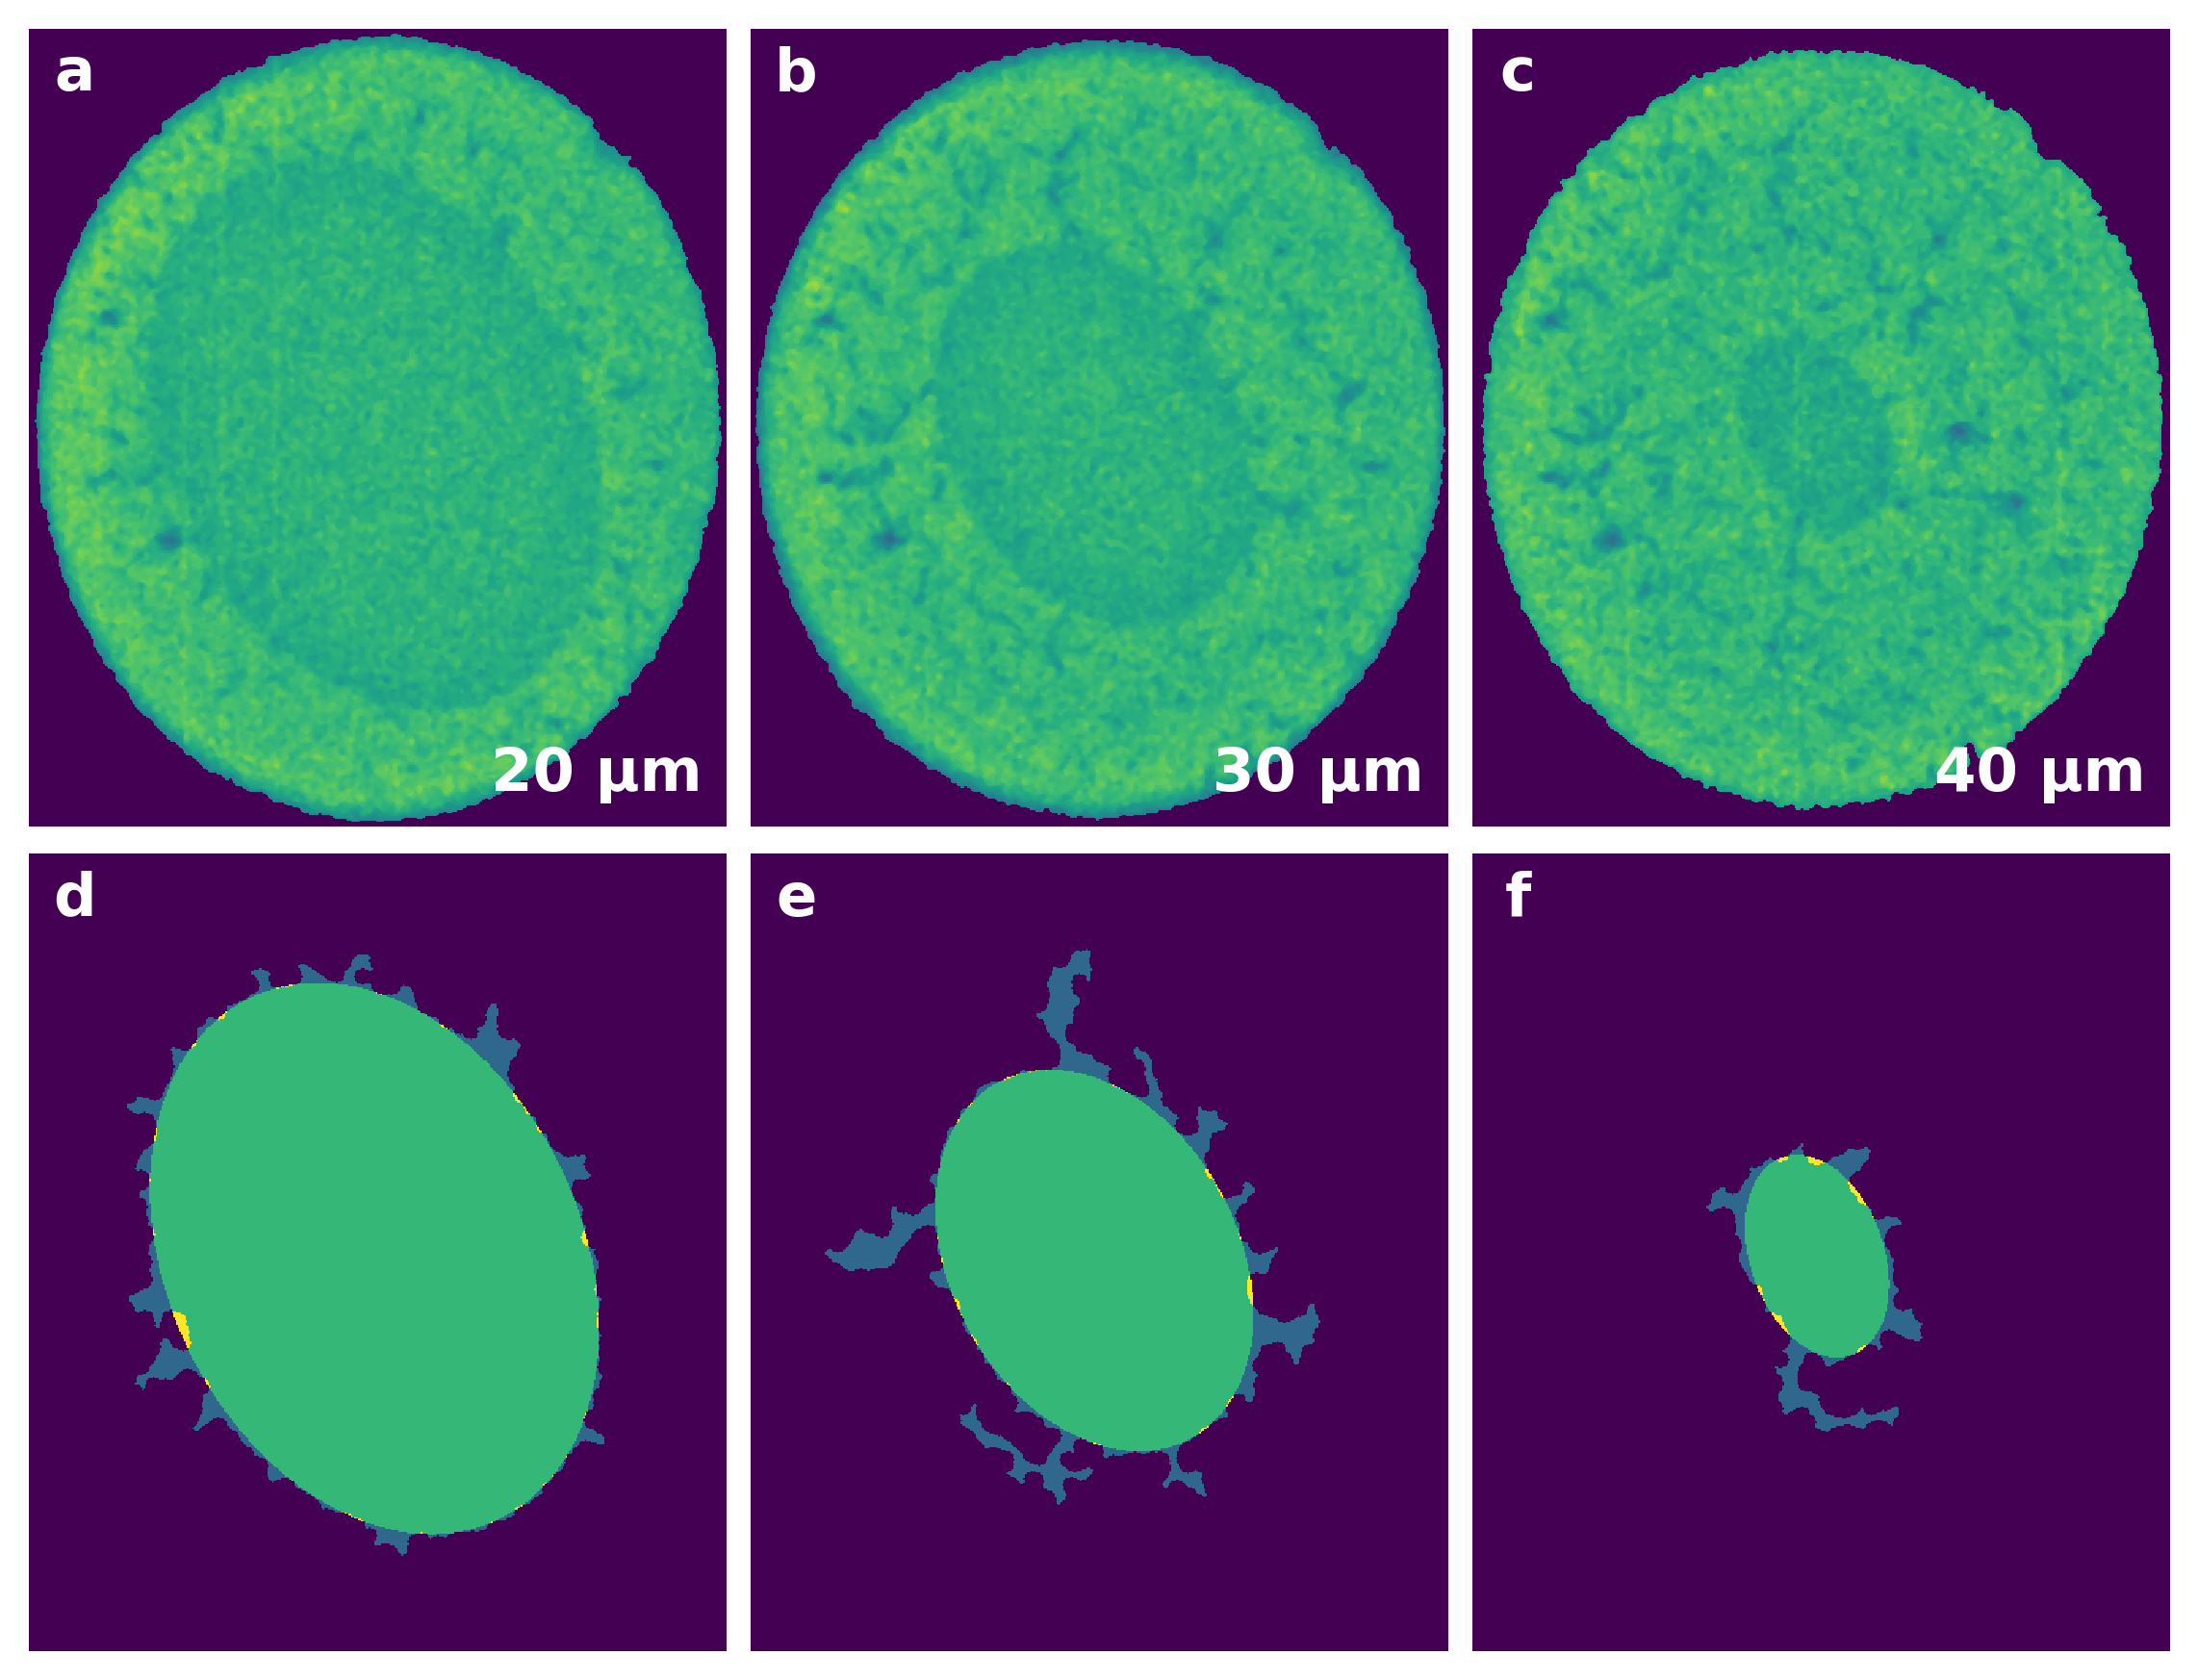
\includegraphics[width=0.75\textwidth]{figures/04/10-rescaled-optim-fit.png}
    \caption{
        \small\setstretch{1}
        (a - c) Subset of normalized frames depicting Al-Si solidification
        20 µs, 30 µs, and 40 µs after the laser melted the sample.
        (d - f) Identified regions overlaid with ellipses of optimized
        fit. Optimization maximizes true fit match (green) and minimizes
        misfit match (yellow) and unfit match (blue). The
        starting point of the optimization are the ellipses of matching
        centroid and second moment (\ref{fig/rescaled-nonoptim}. d - f).
    }
    \label{fig/rescaled-optim}
\end{figure}

The match of the optimized ellipses and the solid-liquid interface of the
experiment can be verified visually by plotting these ellipses on top of
each frame of the solidifying sample (\ref{fig/optim-ellipses}).

\begin{figure}[ht]
    \centering
    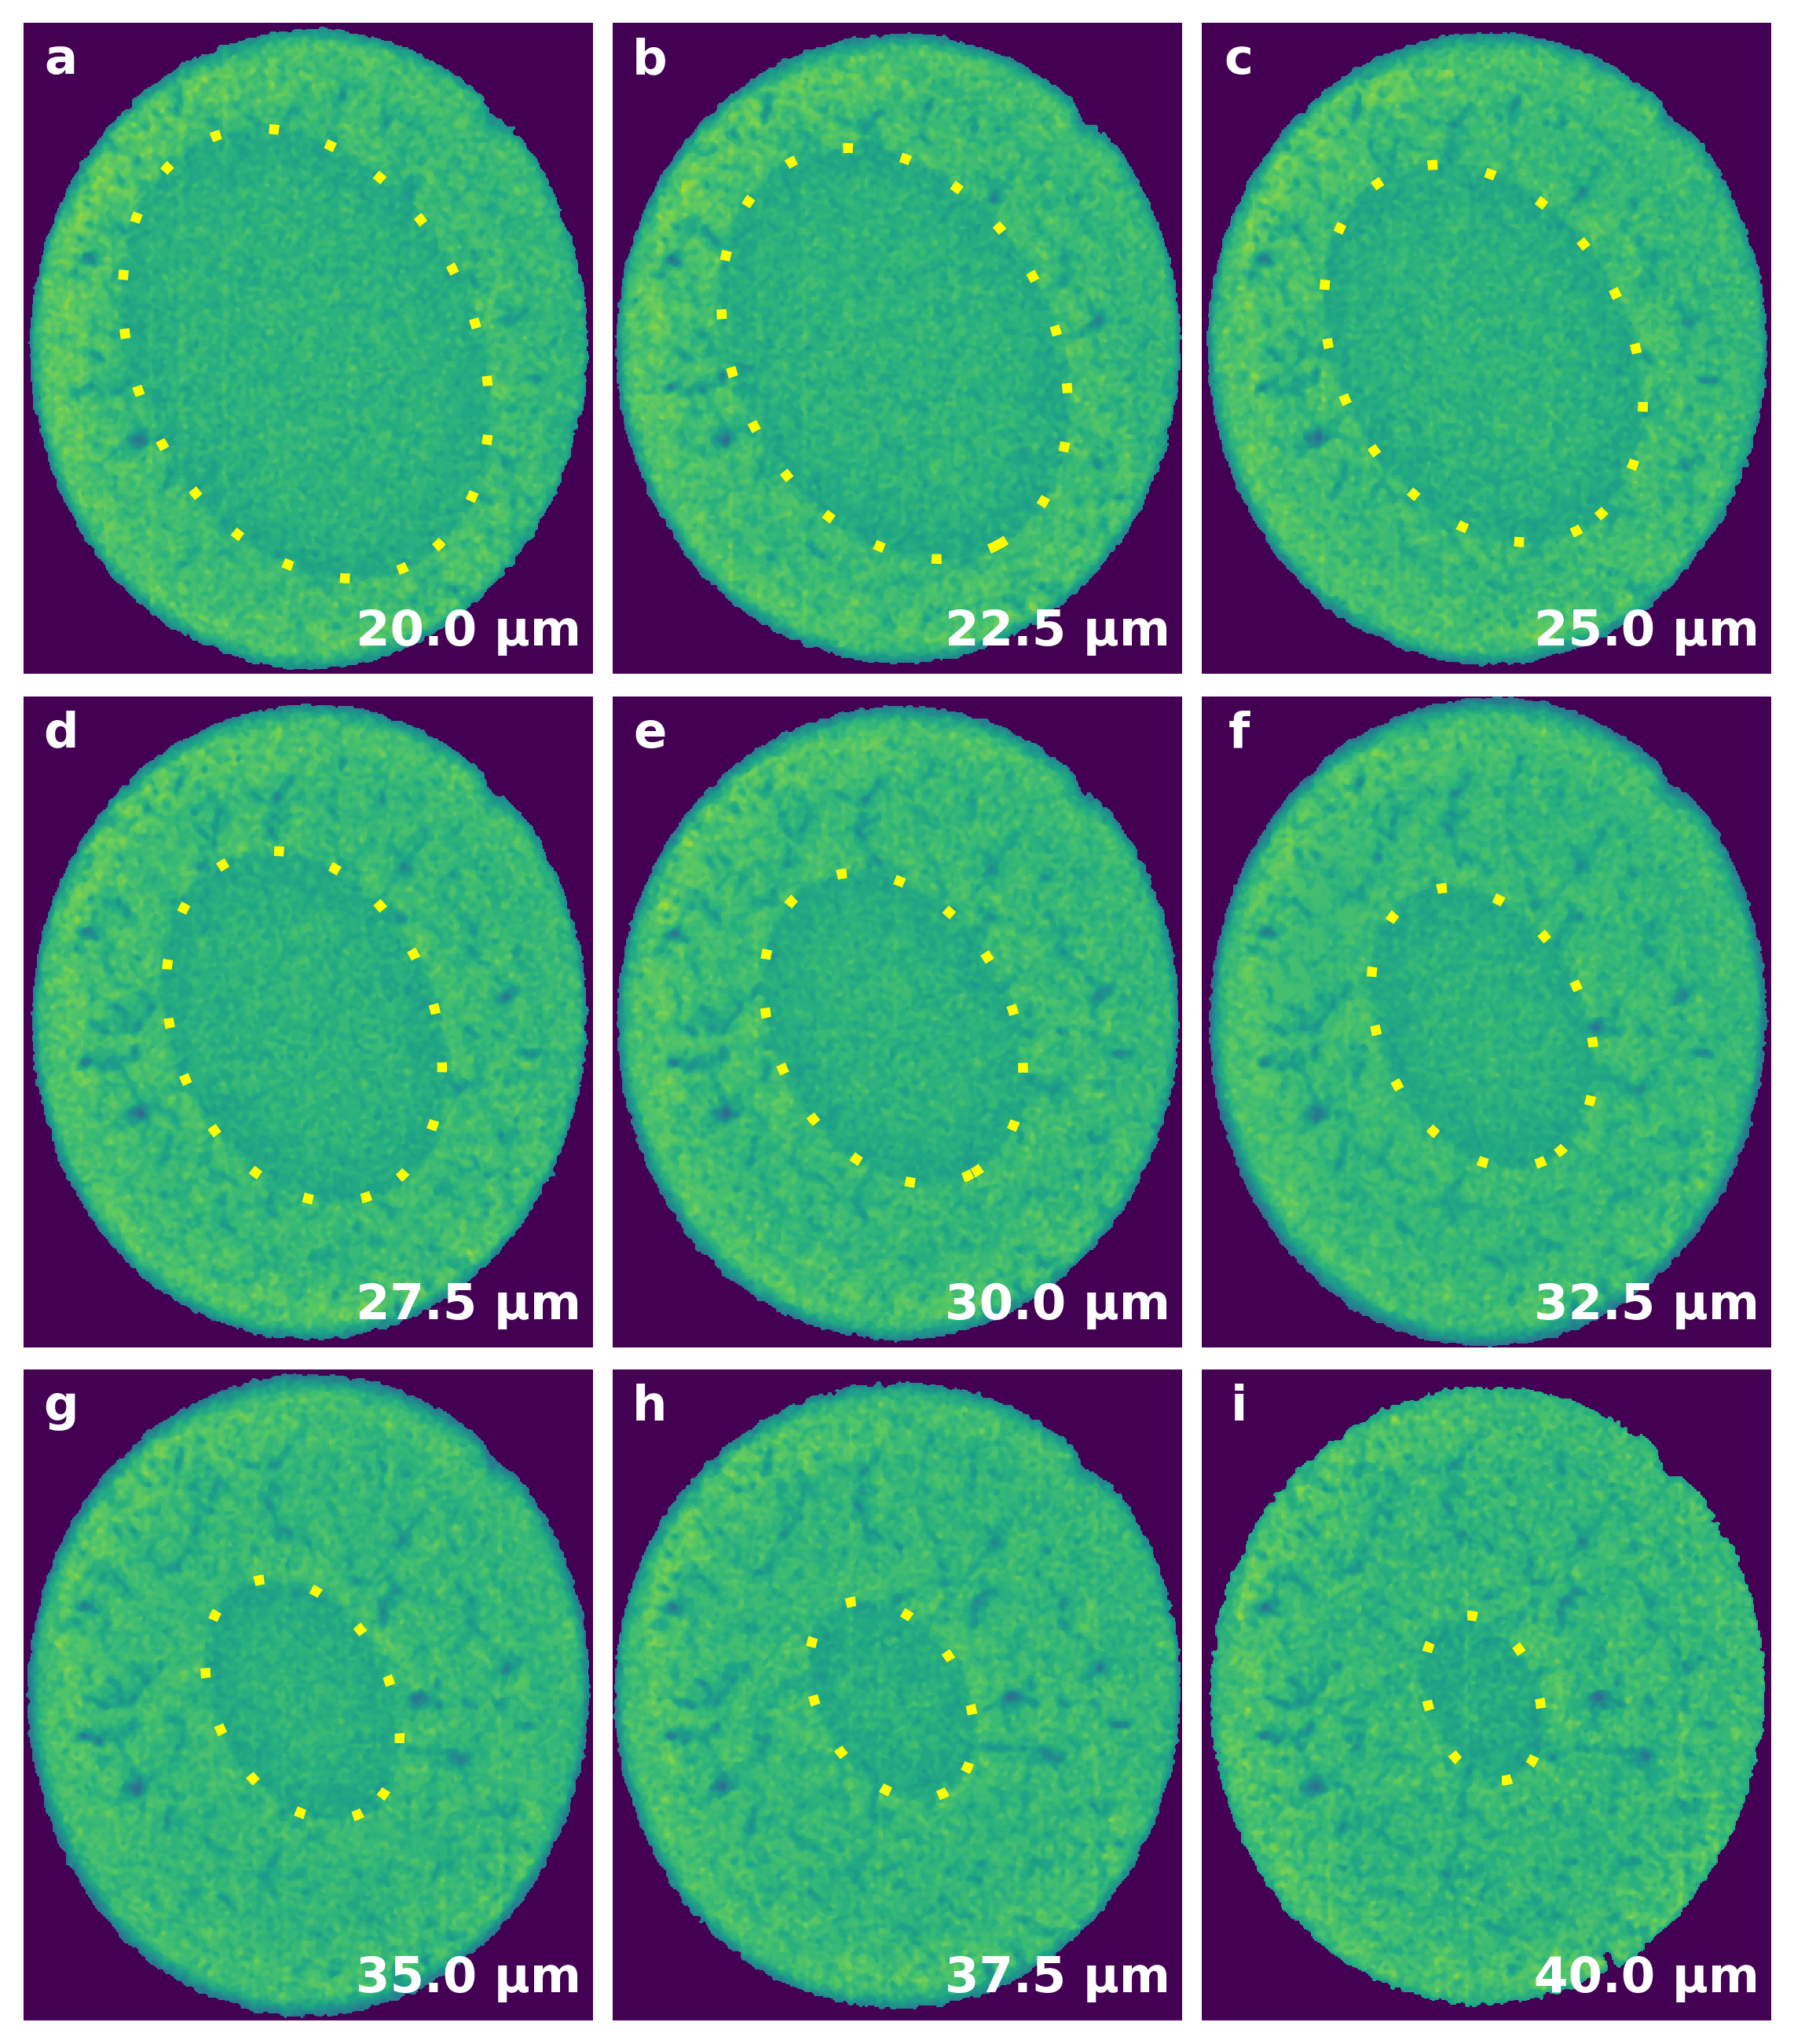
\includegraphics[width=0.6\textwidth]{figures/04/11-rescaled-optim-ellipses.png}
    \caption{
        \small\setstretch{1}
        Optimized fitted ellipses overlaid on each rescaled frame as yellow
        dashed lines.
    }
    \label{fig/optim-ellipses}
\end{figure}

\subsubsection{Rapid Solidification Manual Measurements}
% -------------------------------------------------------------------------
The size of the
optimized ellipses is compared to manual detection of the elliptical
S-L interfaces. A GUI window from the Python package \textit{napari}
was once again used for the manually measurements.
The series of frames segmented from the raw DTEM image was opened in a
\textit{napari} viewer window along with a points layer. A user placed a point
on each side of the long (major) and short (minor) axes of the melt pool.
These line segments define the size of the ellipse and was performed three
times for the DTEM image such that the variance of individual manual
measurements could also be analyzed in addition to the mean
manual measurement when assessing the performance of the detected
interface sizes.

